\chapter{Image Processing}


\section{Definitions and Concepts}
Color Science concerns itself with the characterization of perception of color stimuli, the synthesis of stimuli from perception, and the processing of color information.  Characterization of perceptions from stimuli involves measurement and descriptive processes.  Color reproduction and processing form the basis of most digital applications of color science with the aim to provide a stimulus giving rise to a target perception.  Tristimulus colorimetry is based on three color matching functions which define the primary colors which are mixed to produce a range of stimuli.  The perception of an isolated stimulus is matched to an additive mixture of three light sources called primaries $R, G, B$.  The perception induced by a stimulus is characterized by three values $X, Y, Z$ related to the luminance of the primaries.  Linearly independent light sources are used to create a color measurement system where the tristimulus values encode the amount of each primary required to reproduce a color stimuli.  To calculate a tristimulus value we integrate the spectral distribution of the light source $\phi(\lambda)$ multiplied by the color matching function

\begin{eqnarray*}
\nonumber
  X &=& \int R(\lambda) \phi(\lambda) d\lambda  \\
  Y &=& \int G(\lambda) \phi(\lambda) d\lambda \\
  Z &=& \int B(\lambda) \phi(\lambda) d\lambda
\end{eqnarray*}

\begin{figure}
  \caption{Spectra of CIE Daylight and Fluorescent Illuminants}
  \begin{center}
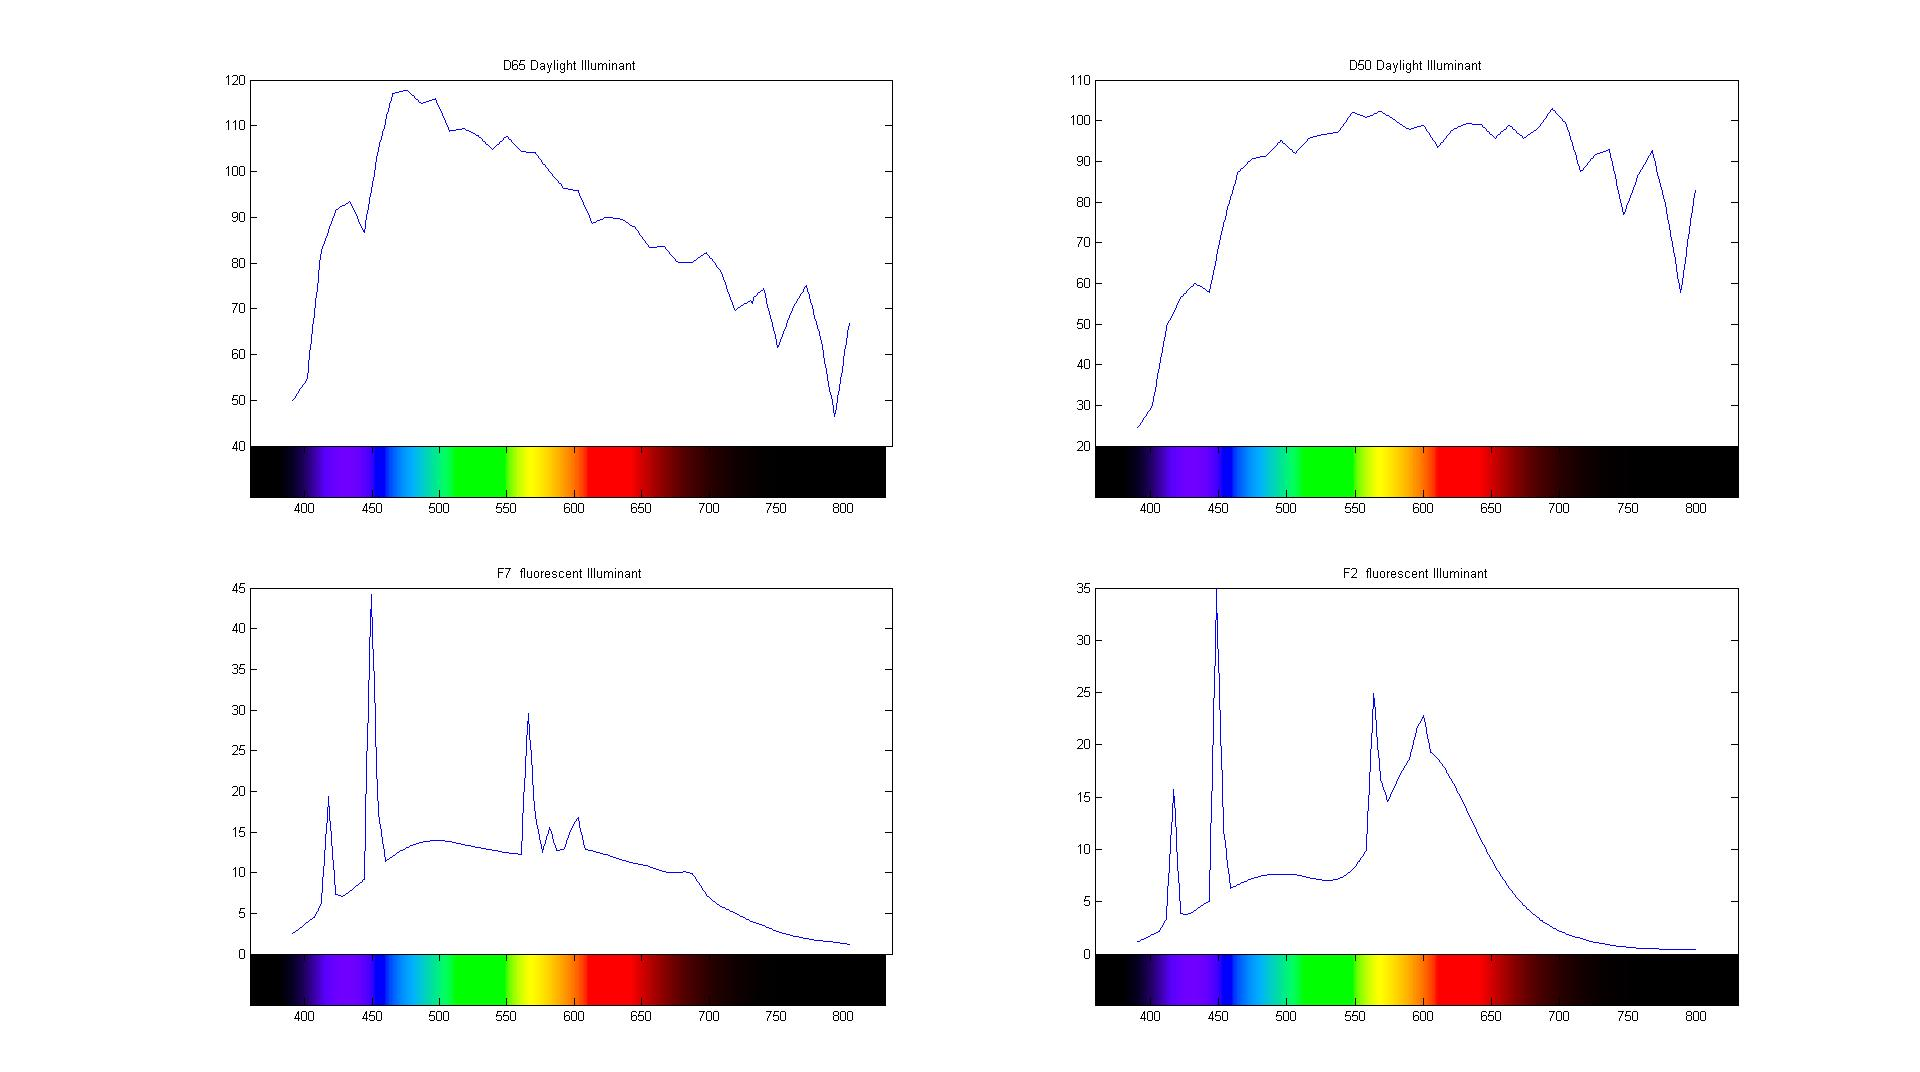
\includegraphics[width=12.0cm]{ColorPaper/daylight_Flourcescent.jpg}
  \end{center}
\end{figure}

\begin{figure}
  \caption{Color Matching Functions for CIE Standard Observer}
  \begin{center}
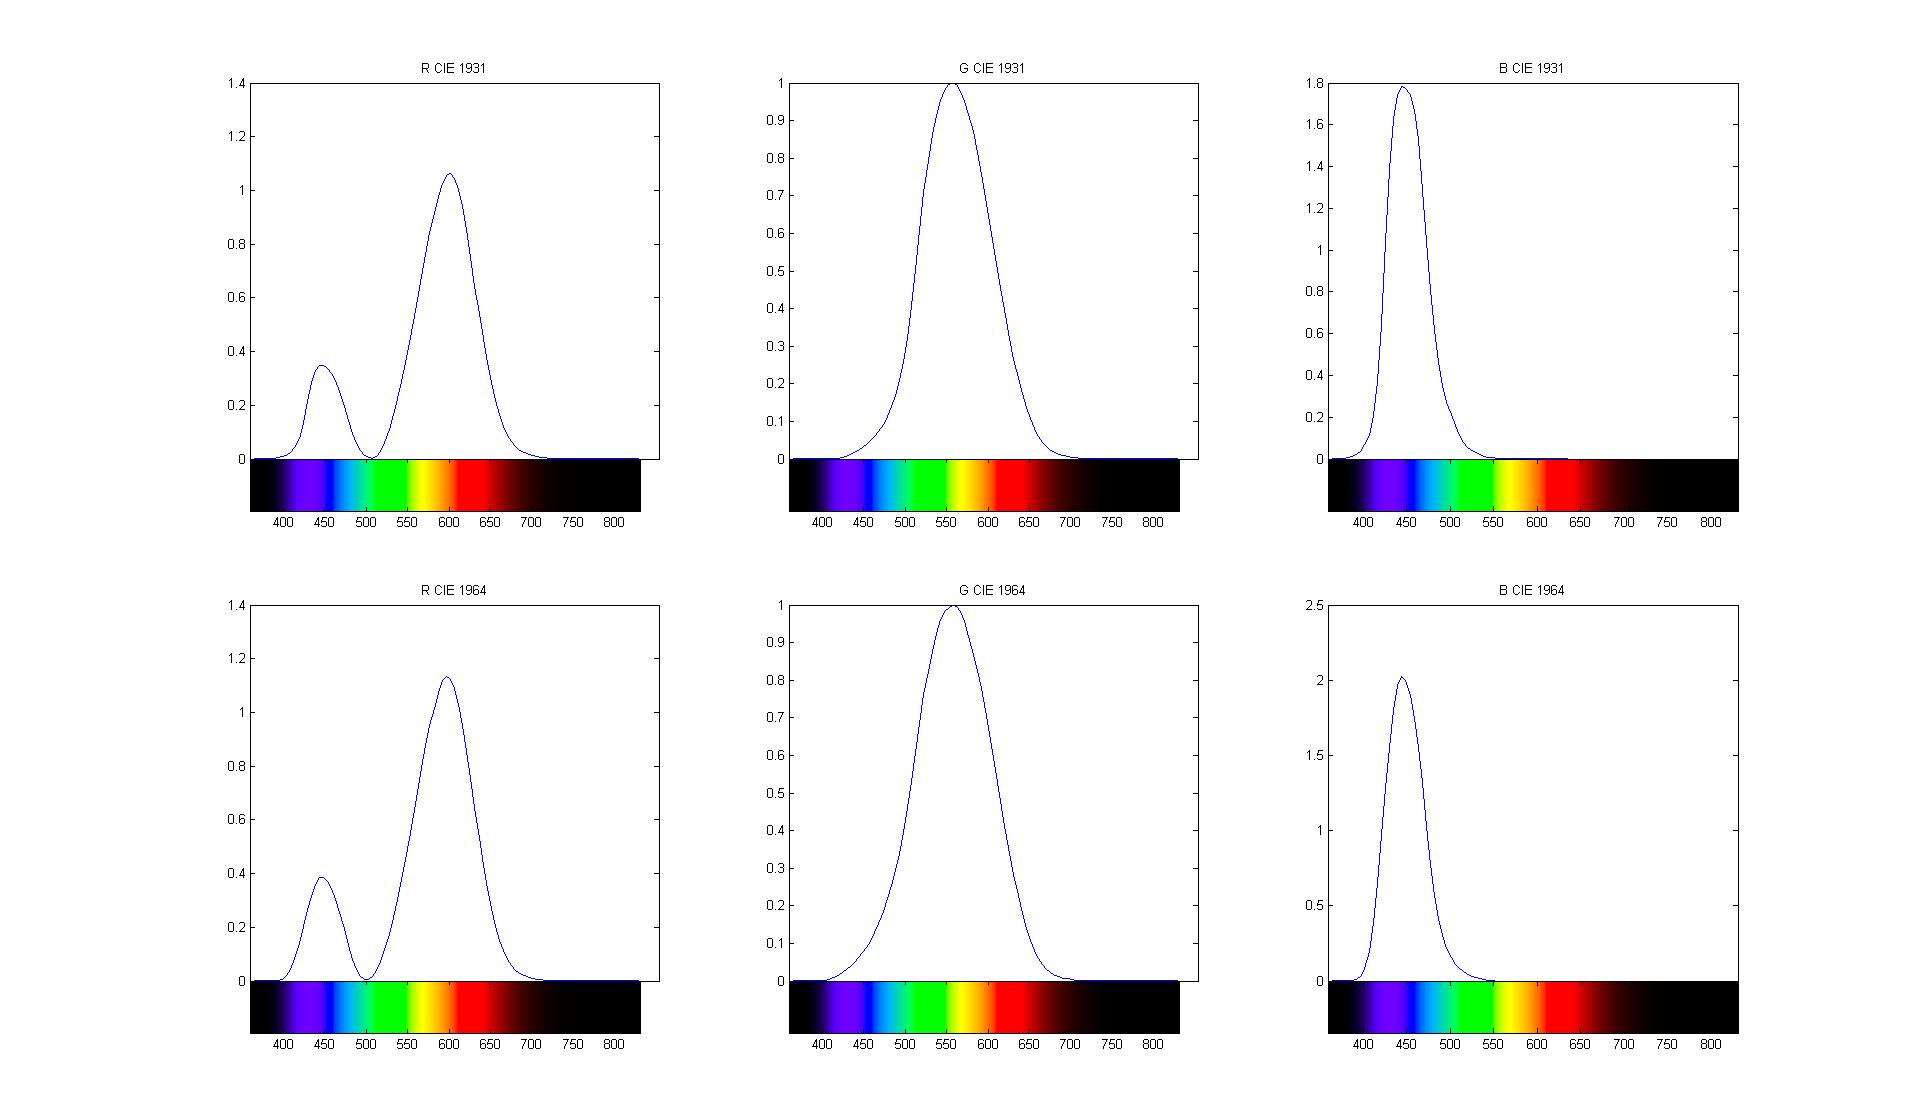
\includegraphics[width=12.0cm]{ColorPaper/XYZ_CMF.jpg}
  \end{center}
\end{figure}
Tristimulus values relate the radiance from a stimulus to the color matching functions.  For color reproduction a set of primaries are fixed and the  tristimulus vector in that color space provides luminances of the primaries required to generate the stimuli.  Color processing is any modification of the color content of a digital image. In order to make the processing task intuitive it has to be done in a representation correlated with the perceptual dimensions of color.  $X, Y, Z$ tristimulus values are not uniform when describing differences in colors.  The CIE Lab color space is a non-linear transform of tristimulus values to a perceptually uniform color space. The transform from tristimulus values to Lab was designed to reproduce the response of the human eye. CIE Lab describes all the colors visible to the human visual system and serves as a device independent color model.  Uniform changes in the Lab color space correspond to uniform changes in color perception.

Chromaticity is an specification of the quality of a color regardless of its luminance. In the Lab color space this is an easy projection on to the ab-plane. The white point of an illuminant is a neutral reference point in the ab-plane.

An absolute color space is one in which which the perceptual difference between colors relates to distances between colors as represented by points in the color space.  Another common definition of an absolute color space is one in which the colors characterized without having to specify an illuminant.
CIEXYZ and sRGB are absolute color spaces. CIE Lab is absolute if one specifies the white point.
There are no simple formulas for conversion between raw RGB values and Lab without the use of an ICC profile or specification of the spectral properties of the primaries and the illuminant.
Converting between non-absolute color spaces or between absolute and non-absolute color spaces has no visual meaning.

An absolute color space can be reversibly converted into another absolute color space but gamut limitations may prevent all of the colors from making the round trip.  Gamut mapping algorithms are typically tuned to preserve application sensitive colors or to minimize overall error.

\subsection{Reflective and Transmissive Models of Color Perception}
The spectral reflectance values obtained from a Macbeth Color chart.

\begin{tabular}{  c c c c }
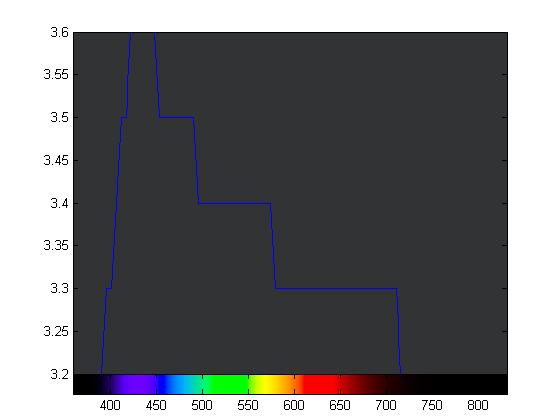
\includegraphics[width=3.0cm,height=3.0cm]{ColorPaper/ch1.jpg}
&
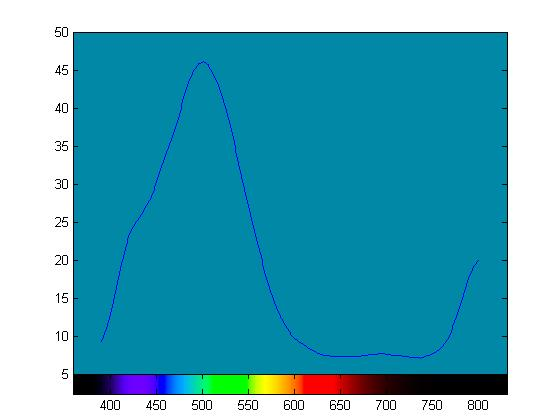
\includegraphics[width=3.0cm,height=3.0cm]{ColorPaper/ch2.jpg}
&
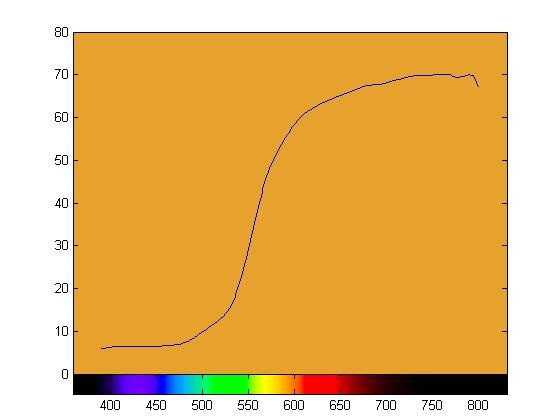
\includegraphics[width=3.0cm,height=3.0cm]{ColorPaper/ch3.jpg}
&
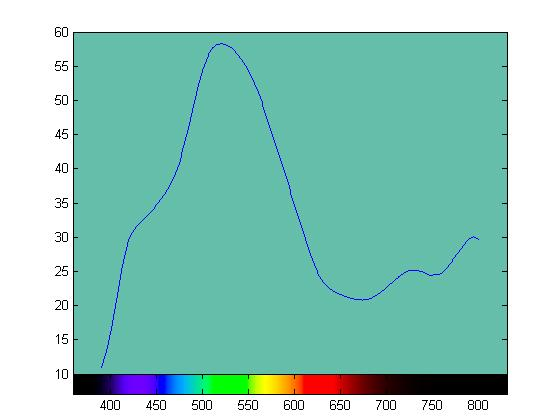
\includegraphics[width=3.0cm,height=3.0cm]{ColorPaper/ch4.jpg}
\\

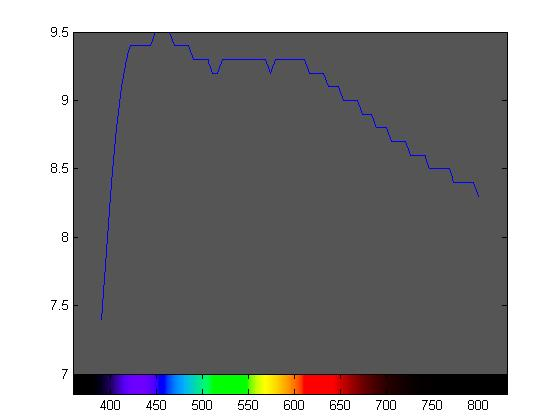
\includegraphics[width=3.0cm,height=3.0cm]{ColorPaper/ch5.jpg}
&
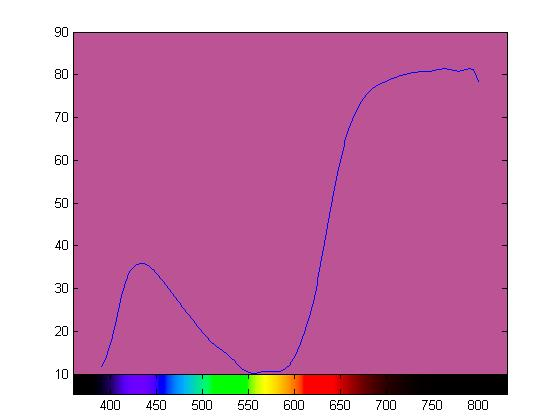
\includegraphics[width=3.0cm,height=3.0cm]{ColorPaper/ch6.jpg}
&
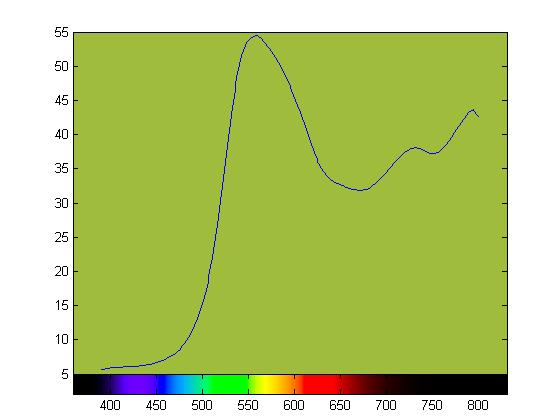
\includegraphics[width=3.0cm,height=3.0cm]{ColorPaper/ch7.jpg}
&
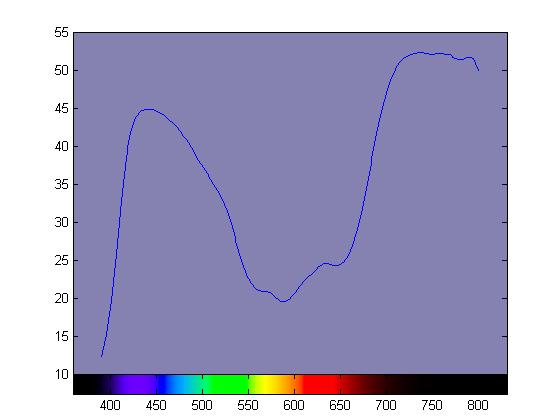
\includegraphics[width=3.0cm,height=3.0cm]{ColorPaper/ch8.jpg}
\\

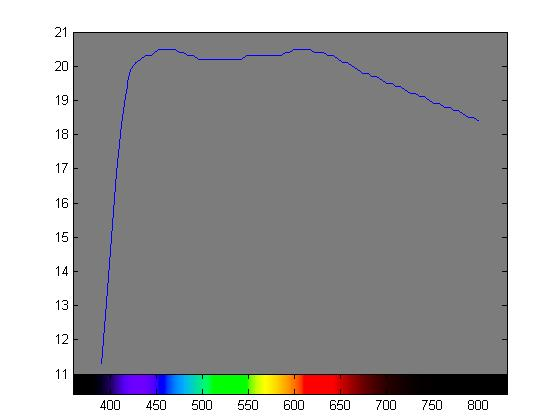
\includegraphics[width=3.0cm,height=3.0cm]{ColorPaper/ch9.jpg}
&
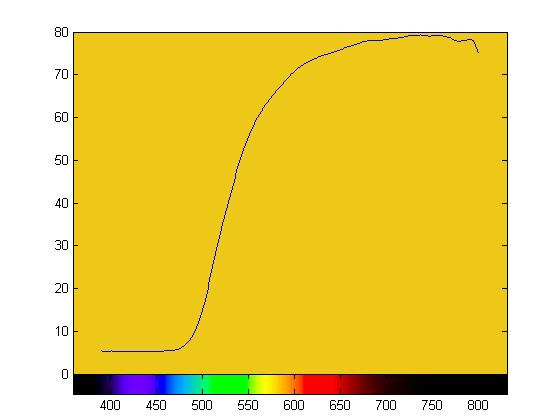
\includegraphics[width=3.0cm,height=3.0cm]{ColorPaper/ch10.jpg}
&
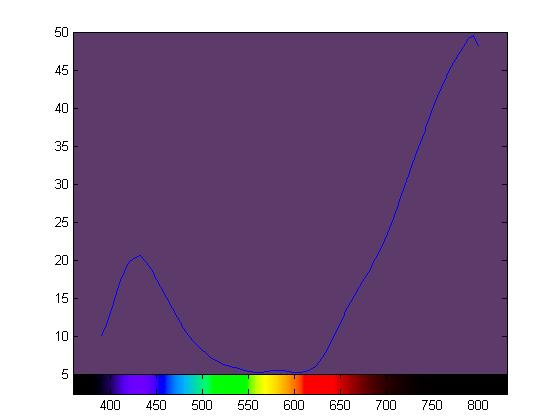
\includegraphics[width=3.0cm,height=3.0cm]{ColorPaper/ch11.jpg}
&
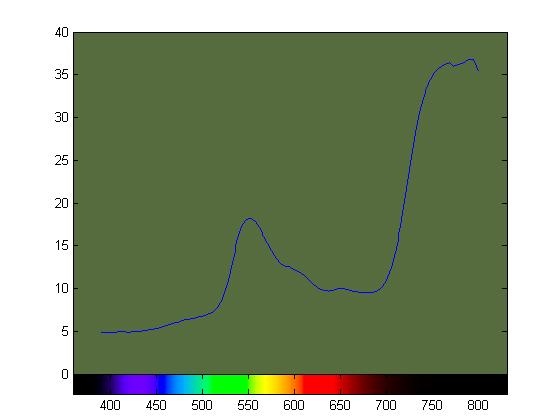
\includegraphics[width=3.0cm,height=3.0cm]{ColorPaper/ch12.jpg}
\\

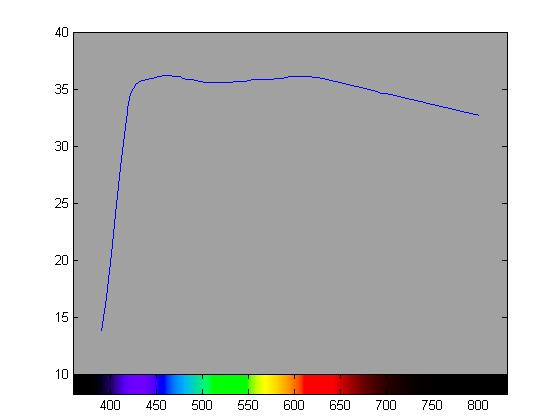
\includegraphics[width=3.0cm,height=3.0cm]{ColorPaper/ch13.jpg}
&
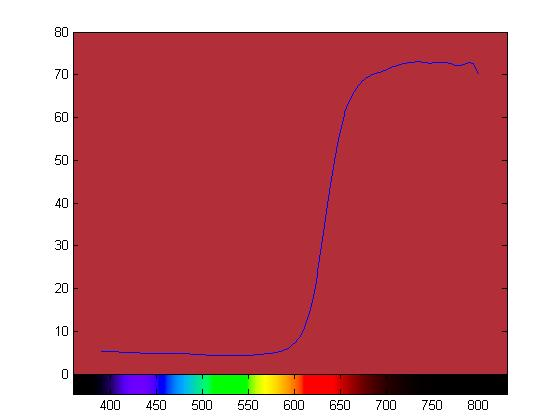
\includegraphics[width=3.0cm,height=3.0cm]{ColorPaper/ch14.jpg}
&
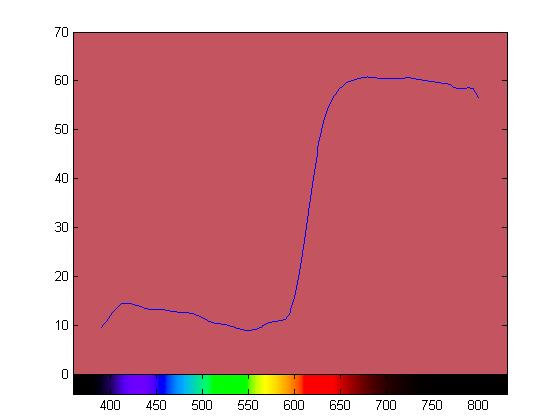
\includegraphics[width=3.0cm,height=3.0cm]{ColorPaper/ch15.jpg}
&
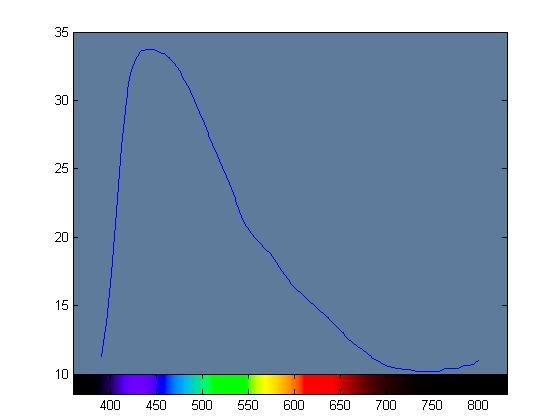
\includegraphics[width=3.0cm,height=3.0cm]{ColorPaper/ch16.jpg}
\\

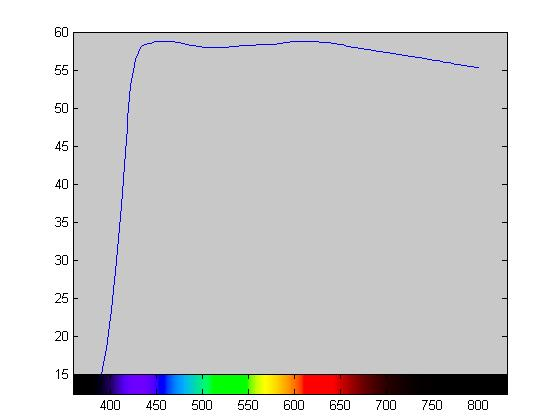
\includegraphics[width=3.0cm,height=3.0cm]{ColorPaper/ch17.jpg}
&
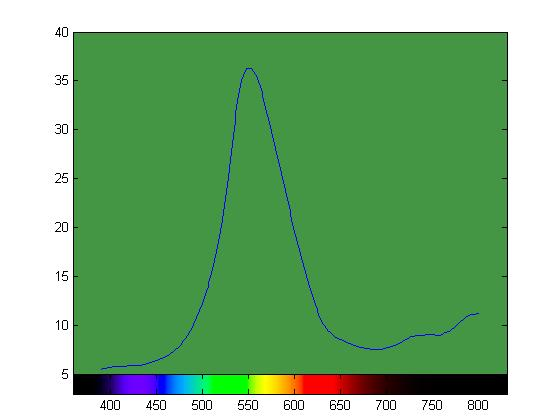
\includegraphics[width=3.0cm,height=3.0cm]{ColorPaper/ch18.jpg}
&
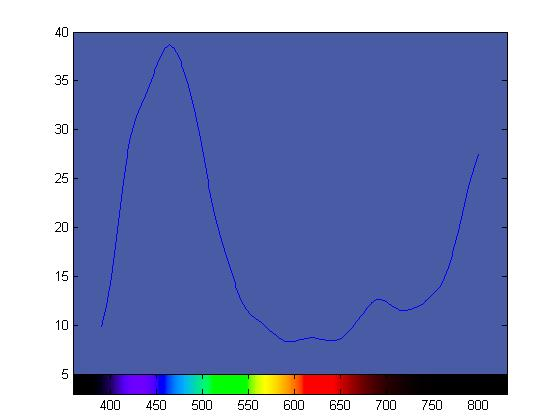
\includegraphics[width=3.0cm,height=3.0cm]{ColorPaper/ch19.jpg}
&
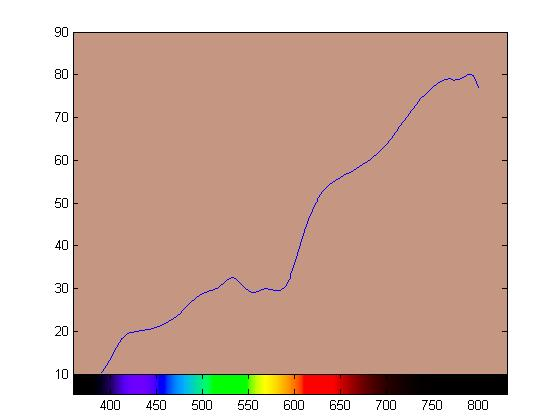
\includegraphics[width=3.0cm,height=3.0cm]{ColorPaper/ch20.jpg}
\\

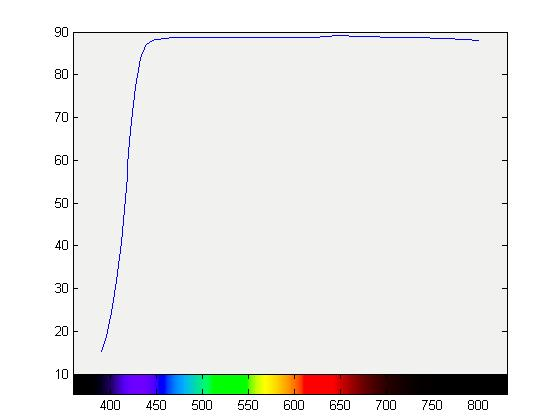
\includegraphics[width=3.0cm,height=3.0cm]{ColorPaper/ch21.jpg}
&
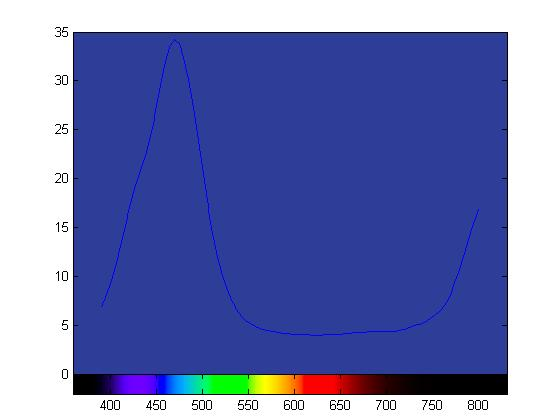
\includegraphics[width=3.0cm,height=3.0cm]{ColorPaper/ch22.jpg}
&
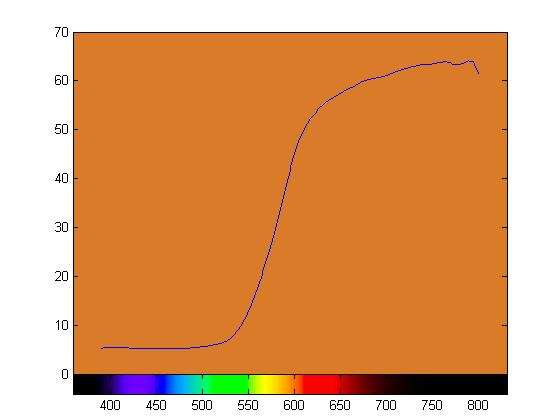
\includegraphics[width=3.0cm,height=3.0cm]{ColorPaper/ch23.jpg}
&
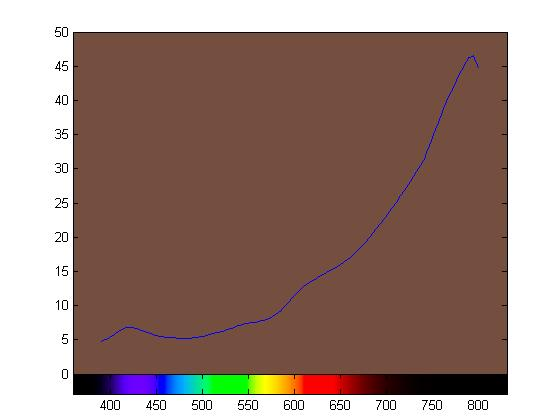
\includegraphics[width=3.0cm,height=3.0cm]{ColorPaper/ch24.jpg}
\end{tabular}

\subsection{Additive and Subtractive Color Models}

\subsection{Gamut Mapping}
Definition definitions used by the CIE TC 8-03 on gamut mapping are given below.

Image: two-dimensional stimulus containing pictorial or graphical information whereby the original image is the image to which its reproductions are compared in terms of some characteristics.

Color reproduction medium: a medium for displaying or capturing color information, e.g. a CRT
monitor, a digital camera or a scanner. Note that in the case of slide scanning, the color reproduction medium is not the scanner but the combination of scanner, stains and glass substrate.

Color gamut: a range of colors achievable on a given color reproduction medium under a given set of viewing conditions.

Color gamut boundary: a surface determined by color gamut extreme values.

Gamut boundary descriptor: an overall way of approximately describing a gamut boundary.
Line gamut boundary: the points of intersections between a gamut boundary and a given line along which mapping is to be carried out.

Color gamut mapping: a method for assigning colors from the reproduction medium to colors from the
original medium or image.

Color reproduction intent: the desired relationship between color information in original and
reproduction media. As a number of solutions to cross-media reproduction intents can be pursued by
gamut mapping. The most generic of these are accuracy and pleasantness but it is also possible to
define others for specific application (e.g. to provide an accurate reproduction of corporate
identity colors while giving pleasant results for others). Note that reproduction intents are also
referred to as rendering intents.

Accurate reproduction intent: aims to maximize the degree of similarity between the original image
and a reproduction of it as far as possible, given the constraints of the color reproduction media
involved. Note that the characteristic of accurate reproduction is intrinsically relative (i.e.
reproduction versus original).

Pleasant reproduction intent: aims to maximize the reproduction�s correspondence with preconceived
ideas of given image should look according to an individual whereby this criterion encompasses
contrast, lack of artifacts, sharpness, etc. Note that unlike accuracy, pleasantness is absolute � at
least as far as given observer understands it at a given moment.

The images below display various perspectives of the gamut of a scanner device [solid] and the sRGB color space [wire].

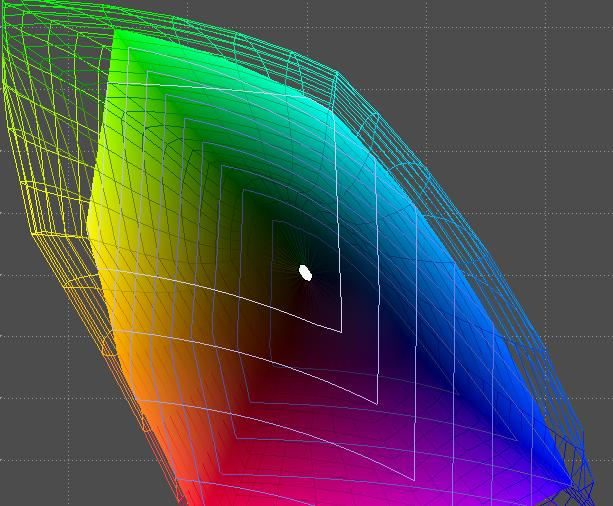
\includegraphics[width=5.0cm]{ColorPaper/aperio_sRGB_v1.jpg}

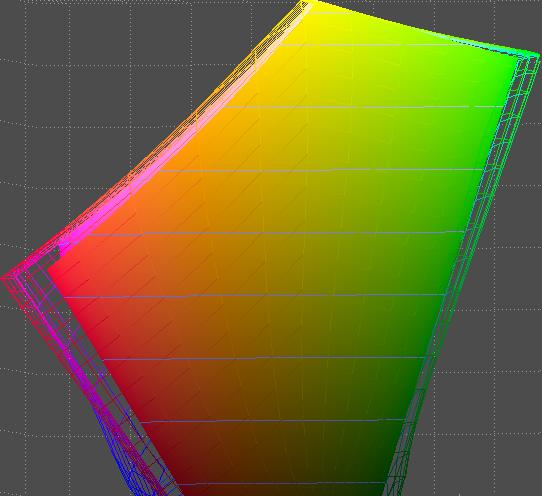
\includegraphics[width=5.0cm]{ColorPaper/aperio_sRGB_v2.jpg}

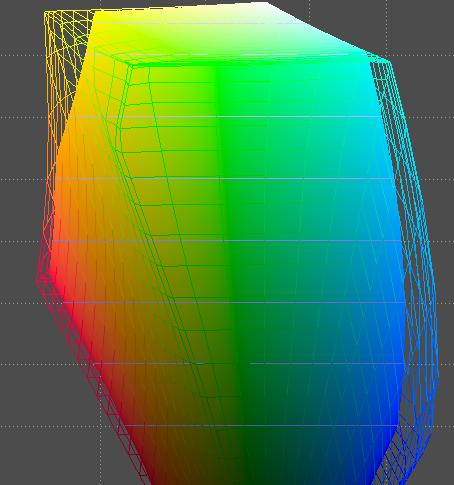
\includegraphics[width=5.0cm]{ColorPaper/aperio_sRGB_v3.jpg}

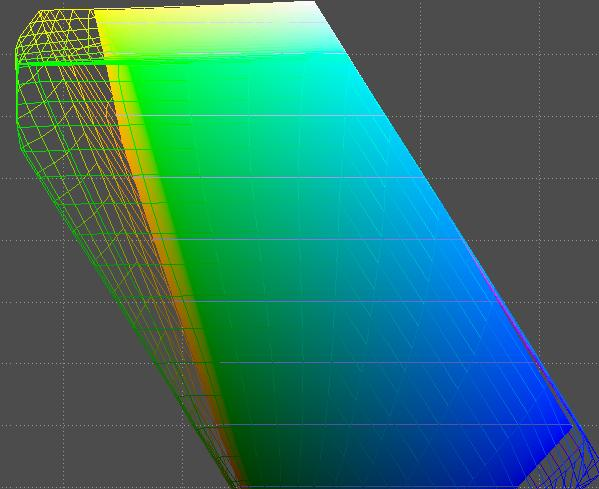
\includegraphics[width=5.0cm]{ColorPaper/aperio_sRGB_v4.jpg}

\subsection{Rendering Intents}
There are 4 rendering intents defined by the International Color Consortium (ICC), which are
specifically defined for the purposes of cross media reproduction using color management
systems. The intents are related to the gamut mapping techniques.

Perceptual intent: the full gamut is compressed to fill the gamut of the destination
device. Gray balance is preserved, the relationship between the colors is not altered
but colorimetric accuracy might not be preserved, as all the colors are moved.
Saturation intent: it converts the saturated colors in the source gamut to the saturated
colors in the destination gamut. This transformation is done at the expense of
accuracy in hue and lightness.

Relative colorimetric intent: only the colors that are outside the destination gamut are
clipped to the destination gamut boundaries. It may result that two different colors of
the source gamut are mapped into the same color in the destination profile. The
relative colorimetric intent takes into account the fact that our eyes always adapt to the white of a medium. The white on the output is the white of the medium and not the
white of the source profile.

Absolute colorimetric intent: it is similar to the relative colorimetric intent except that
the white point of the source and destination are the same. This mode is used for
proofing, where we want to simulate the output of one printer to another device.

\subsection{Affine Transforms of RAW RGB values}
There are a number of non-absolute color transformations that are used in image processing for convenience.  Compression rates in the encoding of JPEG and JPEG 2000 are increased when the RGB values are converted to YCbCr by an affine transform of the RGB values that places most of the color information in the second two components.
These types of transforms are reversible except for floating point roundoff errors.
%\begin{figure}
%  \caption{RGB Cube Transformed to YCbCr}
%  \begin{center}
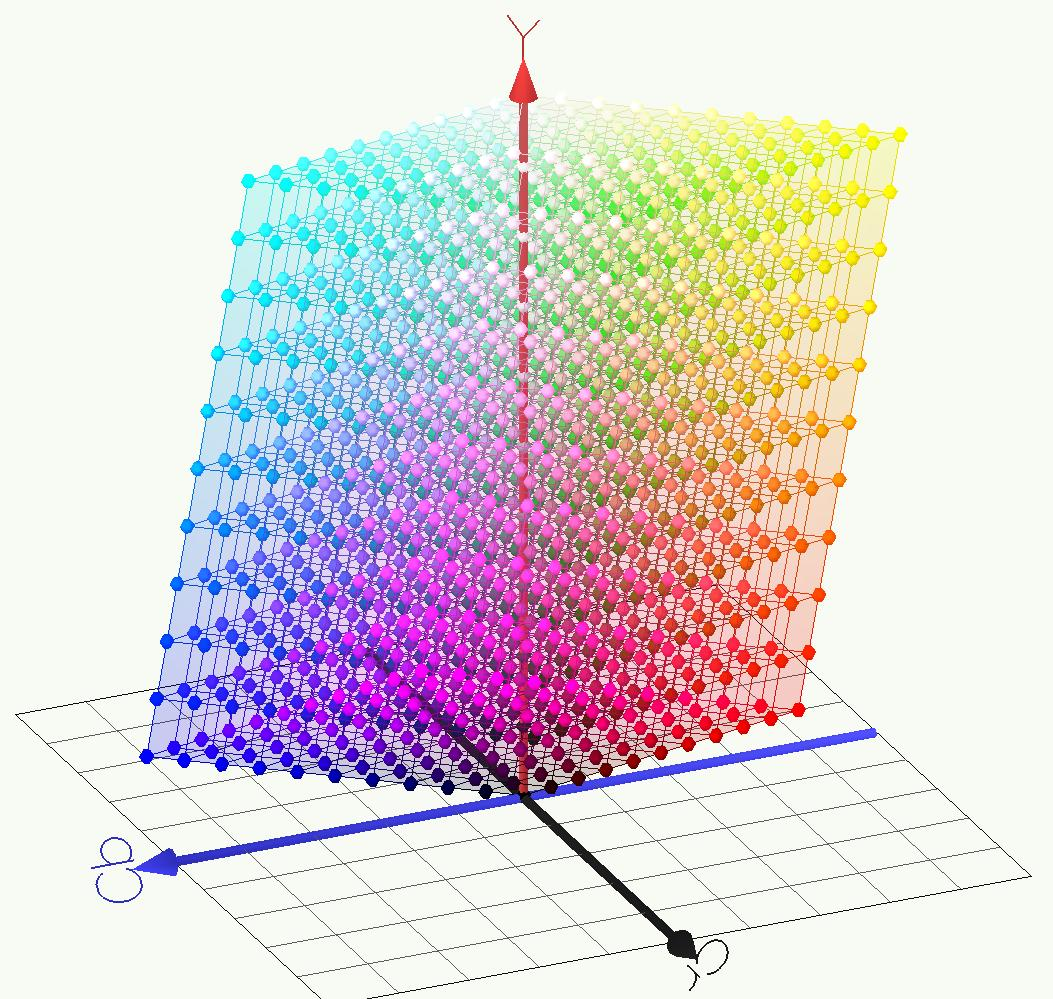
\includegraphics[width=12.0cm]{ColorPaper/RGB_TO_YCBCR.jpg}
%  \end{center}
%\end{figure}

\subsection{Non-Linear Transforms of RAW RGB values}
Color transforms that combine a gamma correction with a rotation of color values are faster that a full gamut mapping transform. The goal of a gamma correction is to obtain an accurate tone scale reproduction.  The associated rotation is usually performed to move luminance data to one channel so that a the non-linear operation takes place in 1 dimension.


\section{Digital Color Management Q and A}
 \begin{enumerate}
 \item
 Light sources are characterized by their spectral power distributions.  The spectral power distribution $\rho(\lambda)$ is the fraction of the total power emitted from a source at wavelength $\lambda$.
 \item
 Daylight is a mixture of direct sunlight, and light that is scattered and diffracted by the atmosphere (skylight).  The power distribution of daylight changes according to weather, time of day, and atmospheric contamination.
 \item
 For the purposes of color measurement, objects are characterized by their spectral reflectance $R(\lambda)$ which is the the fraction of incident light at wavelength $\lambda$ that is reflected from a point on the object.
 \item
 A green object will not always appear to be green.  This can happen under the following circumstances; \begin{itemize}
 \item
 if the spectral power distribution of the light source has low power in the same are of the spectrum where the spectral reflectance is high, then the object will appear to be different from green.
 \item
 if the object is fluorescent and is exposed to a light source that excites the particular wavelength that causes a shift in the reflectance distribution away from green.
 \item
 colorblind observer will not detect a green object to be green.\end{itemize}
 \item
 A color stimulus is a color of light to detected by some observational means.  The color stimulus is characterized by conditions of the light and the objects being observed.  The stimulus at wavelength $\lambda$ is the product of the spectral power distribution of the light source and the spectral reflectance of the object; $S=\rho(\lambda)*R(\lambda)$
 \item
 The human audio and visual systems are fundamentally different in terms of frequency domain processing and the spatial resolution capability. Spatial location of a stimulus is much better with the visual system.  The audio system is capable of decoding and resolving any waveform with frequency components less than about 26kHz using a single detector.  The human visual system uses three different receptors for light. These detectors have some overlap in their sensitivities - the overlap in the sensitivity gives some degree of freedom to the resolving process. It's under-determined, so there are multiple inverse solutions to a particular measurement of a stimulus - $M(S)$ - to the human visual system. This property is called metamerism.  An imaging system may be able to resolve stimuli that the human visual system can distinguish, this can complicate output if not handled. Metamerism simplifies imaging systems because it reduces the number of colors that must be faithfully reproduced.  Some imaging systems get by with 256 colors - down from the 11 million that can be detected by the human visual system.  Think of this as a lossy compression/decompression.
 \item
 Objects may not appear the same under differing light sources because of metamerism.  The stimuli might be the same for both under one light source even though the reflectance differs. Changing the light source changes $\rho(\lambda)$ which may elicit different stimulus responses $S$for the two objects.
 \item
 Colorimetry is the process of encoding and measuring colors for retrieval and display in imaging systems.
 \item
  True or false: The spectral responses of the CIE standard observer are identical to the cone responses of the average human observer. "   Why, or why not?
 \par  False.  The CIE trichromatic color matching functions are a linear combination of any average cone response functions.
 \item
 What information is needed to compute CIE tristimulus values?
 \par The spectral power distribution of the light source \(S(\lambda)\), the spectral reflectance of the object,\(R(\lambda)\), the CIE color matching functions; \begin{math}\overline{x}(\lambda),\overline{y}(\lambda),\overline{z}(\lambda) \end{math}, and a normalizing constant are integrated over \( \lambda \) in \( [380,780] \). \begin{eqnarray} \nonumber X = \int R(\lambda) S(\lambda) \overline{x}(\lambda) d\lambda \\ \nonumber Y = \int R(\lambda) S(\lambda) \overline{y}(\lambda) d\lambda \\ \nonumber Z = \int R(\lambda) S(\lambda) \overline{z}(\lambda) d\lambda \end{eqnarray}
 \item
 Would it be possible to build an output device, such as a video projector, using the primaries defined in the CIE XYZ system? " Why, or why not?
 \par No.  The primaries in the CIE XYZ system were chosen to give the color matching function non-negative values.  This requires the primaries to have negative power in some region of the spectrum, which can't really be realized in a light source.
 \item
 What does a CIE x, y chromaticity diagram show? "   What does it not show?
 \par If the $X, Y, X$  tristimulus values are normalized , the plot of $X/(X+Y+Z), Y/(X+Y+Z)$ gives the qualities of a color stimulus with the luminance normalized out.
 \item
 True or false: The appearance of a color can be described by a set of CIE X, Y, Z tristimulus values.\par False.  The CIE coordinate system is useful for describing color differences for small differences in stimuli, but not for describing the appearance of a color.
 \item
 True or false: The appearance of a color can be described by transforming its CIE X, Y, Z tristimulus values to CIELAB or CIELUV color space.
 \par  False.   The appearance of a color is dependent on the viewing conditions.  CIELAB and CIELUV color spaces are good for measuring differences in color.
 \item
  Describe an appropriate use for a Status A densitometer. Describe an inappropriate use for a Status A densitometer.
 \par  An appropriate use of a Status A densiometer would be to measure or to monitor the optical density of the output of a three channel imaging system.  An inappropriate use would be to do colrimetry calculations base on desiometer readings.  The Status A densiometer response functions are tuned to the narrow bandwidth supported by dyes.  Also using the Status A readings to compare output from different imaging systems is not advised.  The Status A readings from different systems may agree, but that does not imply the systems generate images with the same appearance.
 \item
 What are the three basic functions required in all imaging systems? · Define each of these functions.
 \par Capture, signal processing, and image formation.  Capture is the process of detecting light stimuli from a scene.  Signal processing is modifies the captured image for output.  Image formation takes the processed signal and uses it to control the color forming elements of the output device.
 \item
 Why is color separation trichromatic in most color-imaging systems? · Describe an application in which color separation other than trichromatic might be required.
 \par Most color imaging systems are trichromatic because the human visual system is.  X-ray capture is monochromatic, and some landsat imaging imaging systems may have more than three bands of capture.
 \item
 How can color separation be accomplished in an electronic camera?
 \par Color separation in an electronic camera may be achieved by capturing image data on a CCD mosaic of RGB sensors.  Light can also be optically separated into three bands and then sent to three different CCD sensors - one for each band.
 \item
 How is color separation accomplished in photographic films?
 \par Color separation in photographic film is done through three or more light sensitive layers and filters.
 \item
 What is meant by exposure factor? · How can exposure-factor values be calculated?
 \par The exposure is calculated by integrating the spectral responsivity with the light spectrum and the spectral reflectance or transmittance of the object being imaged.
 \item
 What is the basic function of color signal processing? · Describe some of the transformations typically included in color signal processing.
 \par The basic function of color signal processing is to make an image suitable for viewing.  Typical functions are signal amplification, non-linear modification of the neutral signal, and color matrix calculations, sharpening and noise reduction, and possibly compression.
 \item
 What are the two basic types of color image formation? · Are other types of color image formation possible? · If so, describe at least one.
 \par The two basic types of color image formation are additive color mixing and subtractive color mixing.  Other types are possible.
 \item
 In an additive system, what color is formed by: · Red and blue? · Blue and green? · Red and green? · Red plus green and blue?
 \par In an additive color forming system, red and blue make magenta, blue and green make cyan, red and green make yellow, and red plus blue plus green make white.
 \item
 In a subtractive system, what color is formed by: · Cyan and yellow? · Yellow and magenta? · Magenta and cyan? · Cyan plus magenta and yellow?
 \par In a subtractive color forming system, cyan and yellow make green, yellow and magenta make red, magenta and cyan make blue, and cyan plus magenta plus yellow make black.
 \item
 Define a complete color-imaging system. · Is a digital camera a complete color-imaging system? Why, or why not? · Is a photographic slide film a complete color-imaging system? Why, or why not?
 \par A complete color imaging system is one that can perform capture, signal processing, and image formation.  A digital camera is such a system.  Capture and signal processing take place in the camera, and image formation takes place on the LCD screen on the back.  Photographic slide film is a complete color imaging systems well.  Capture takes place in the camera, signal processing and image formation takes place in the lab.
 \item
 Describe an application in which an instrument, such as a colorimeter, would be preferred for assessing color quality.
 \par A colorimeter would be used to compare an original scene to a reproduction produced by a color imaging system.
 \item
 Describe an application in which a human observer would be preferred for assessing color quality.
 \par Taking a picture with photographic film, and then viewing the reproduction later.
 \item
 What aspect of the human visual system corresponds to: · image capture · signal processing · image formation
 \par Image capture takes place in the rods and cones of the eye, signal processing and image formation both take place in the brain.
 \item
 What is psychological signal processing?
 \par Psychological signal processing is the component which accounts for color memory, and color preference.
 \item
 What is psychophysical signal processing?
 \par Psychophysical signal processing is the component of image processing in the human brain which takes into account effects like chromatic adaptation, lateral brightness adaptation, and the relative nature of luminance detection.
 \item
. Define each of the following: · general-brightness adaptation · lateral-brightness adaptation · chromatic adaptation
 \par Brightness adaptation is how the eye responds to varying levels of illumination.  Lateral brighness adaptation is how the eye has different sensitivities in different parts of the eye. Chromatic adaptation is how the eye responds to an average chromatic stimulus of a scene.
 \item
 For each adaptation effect listed in question 6, give an example of how the effect might be encountered in a practical imaging situation.
 \par Brightness adaptation would be encountered when viweing conditions change from low to high light illumination.  Lateral brightness adaptation would be encountered when focusing on different objects - closer objects are captured with the fovea. Chromatic adaptation occurs in incandecent illumination induces an increase in short wavelenght sensitivity.
 \item
 Describe the relationship of CIE colorimetry to human color vision. · What aspects of color vision are predicted well by standard CIE colorimetry? · What aspects are not predicted well? Why not?
 \par CIE colorimetry can be used to predict if two stimuli will visually match under identical viewing conditions.  CIE colorimetry can not be used to emulate signal processing of color formation functions.
 \item
 For the purposes of color characterization, what characteristics of a color monitor must be measured or otherwise determined?
 \par The CIE x,y chromaticity coordinates of the monitor red, green, and blue primaries must be determined experimentally, or be given by the manufacturer.  The location of the chromaticity coordinates determines the gamut of colors the monitor can produce by adding varying intensities of the red, green, and blue primaries. The color matching functions of the CIE standard observer can be obtained from the x,y chromaticity coordinates of the primaries.
 \item
 What does “monitor white point” mean?
 \par The monitor white point is the chromaticity coordinates of the stimulus obtained by mixing the red, green, and blue primaries at full intensity - $ (R,G,B)=(255,255,255) $ for an 8 bit monitor.
 \item
 What does “monitor grayscale tracking” mean? · Why is such tracking important?
 \par Monitor greyscale tracking is the ability to emit light of constant chromaticity but varying luminance when $R=G=B$.
 \item
 Monitor and hardcopy images are said to be “highly metameric”. · What does this mean? · Describe a practical consequence of a high degree of metamerism. · Describe a method for dealing with that consequence.
 \par For a monitor to reproduce a color stimulus with a monitor we add light from three sources.    Metamerism is when the spectral power distribution of the light source produced by the monitor is very different from the spectral power distribution of the stimulus - even though the CIE tristimulus values of the two stimuli are the same.  The spectral power distribution of the three sources determine the amount of each light source needed to produce a particular stimulus.  For hard copy the spectral reflection density of the dye set used for the print is what determines the amount of each dye to use for a given stimulus.  Because of the differences among individual responsivities differ from the CIE standard observer, two individuals observing a color on the monitor may disagree whether the stimulus matches a reference one.  Color matching experiments can be done for each observe to correct for this.
 \item
 Why should (or should not) logarithmic units be used in characterizing the grayscales of monitors?
 \par Taking the log of monitor luminance gives a better measure of differences at the low end of the luminance scale. The CIE L-a-b luminance is defined as  $L^{*}=116 (\frac{Y}{Y_n})^{\frac{1}{3}} -16 $.  Conveniently, the ...
 \item
 What grayscale characteristic must a video camera have for the entire system to have a grayscale that is one-to-one with that of the original scene?
 \par The greyscale characteristic of the camera needs to be the inverse of the greyscale characteristic of the monitor.
 \item
  In addition to an appropriate grayscale characteristic, what further characteristic must a video camera have for the entire system to have colorimetric color reproduction that is one-to-one with that of the original scene? \newline
 \par The chromaticities of the non-neutral scene colors must match the output device chromaticities. \newline
 \item
 Describe the appearance of such colorimetric color reproduction. \newline
 \par When the chromaticities of the input match those of the output device, the result is something the viewer would report as being less saturated than the original scene. This is because using the CIE standard observer color matching functions as camera sensitivities leads to chromatic errors. Since the CIE Standard Observer color matching functions are a linear transform of any other color matching functions, we can remove these errors by transforming the camera color matching function from the ones representing the monitor primaries to another set that accurately reproduces the color stimuli. \newline
 \item
  What additional factors must be taken into account in order to produce pleasing reproductions of original scenes? \newline
 \par In addition to accurate colorimetric reproduction, psychophysical effects of the human visual system must be taken into account in order to produce visually pleasing results. \newline
 \item
  How can video signal processing be used to account for these factors? \newline
 \par The greyscale characteristic can be modified to account for viewing flare.  Also, the reproduction device is of a lower overall luminance than the original scene - which leads to a reduction in the perceived saturation.  Boosting the greyscale characteristic accounts for this effect as well. \newline
 \item
 Describe the principal components of an ideal video system. · How do practical systems correspond to this ideal? · Why will the color gamut of any real CRT be limited? \newline
 \par An ideal video system would have camera spectral sensitivities with all positive color matching functions so that all color could be realized by the monitor.  There should be a color matrix transformation that converts the camera color matching functions to ones that correspond to the monitors.  The gamut of a monitor will be limited because the transform from the CIE standard observe to monitor color matching functions will give colors with negative amounts of monitor RGB primaries.  The CIE standard observer color matching functions were all positive, and all colors could be reproduced because the primaries were imaginary.  The monitor primaries are not imaginary - this is the reason why the color matching functions of the monitor must have negative values. \newline
 \item
 Describe three possible methods for encoding video signals. \newline
 \par We could just do the colorimetric matching.  We could do the color matching and then let Ed tweak the signal processing so the results are pleasing.  Lastly we could reverse engineer any imaging system to produce pleasing results - get data on the output, and taylor the signal processing to produce the characteristics the viewers have reported as pleasing.  This last suggestion works for any given imaging system, but we would not be able to design the signal processing of an input or output device in isolation this way.
 \item
  What general characteristics are shared by virtually all reflection media? \newline
 \par  Most reflection-print media consist of three or more subtractive dyes used to form an image on some type of reflective support material. \newline
 \item
  What happens when a ray of light strikes the surface of a simple reflection medium? \newline
 \par Some incident light will be reflected on the surface of the media, the rest will be refracted through the colorant layer and scattered off the reflective support. Some light scattered off the support will be reflected off the surface coating back to the colorant. \newline
 \item
  A neutral object is photographed under a first illuminant. A reproduction is made and viewed under a second illuminant. For the reproduction of the object to appear neutral, should its chromaticity match that of the first illuminant or that of the second illuminant? Why? \newline
 \par The chromaticity of the reproduction neutral should be the the chromaticity of the illuminant the reproduction is viewed in.  The observer will be chromatically adapted to the second illuminant when viewing the reproduction.  If the chromaticity of neutral objects are reproduced with the chromaticity of the first illuminant, the observer will perceive the difference. \newline
 \item
  What is meant by “viewing illuminant sensitivity”? Why it is important in imaging applications? \newline
 \par Viewing illuminant sensitivity is a measure of how much image dye components must be modified to produce a metamer when reproducing neutrals to be viewed under different illuminants.   This is important in imaging systems because the same reproduction could be viewed under different illuminants, and the observer may perceive a difference under the two illuminants if the viewing illuminant sensitivity is high. \newline
 \item
 Why would the grayscale characteristic of a reflection-print system not be one-to-one with the original scene? \newline
 \par If the viewing conditions of the scene are different from the viewing conditions of the reproduction, the grayscale would need to be modified.  The contrast is boosted for the midrange and rolled off at the ends of the density range.  This is done to accommodate for viewing flare and differences in the absolute luminance of the scene and the viewing environment of the reproduction.
 \item
  System A has a higher maximum density and a lower minimum density than System B. Which system will require a higher mid-scale gamma? \newline
 \par The dynamic range of system A is greater than system B.  The midscale gamma of system B will need to be higher to produce dark and light tones at acceptable density.
 \item
  If the taking illuminant and viewing illuminant of a reflection-print system differ in chromaticity, what is required in order to make a meaningful evaluation of reproduced chromaticity values? \newline
 \par The observes state of chromatic adaptation in the viewing environment must be taken into account. \newline
 \item
  Why might the reproduced colorimetry of a reflection-print system differ from that of an original scene? \newline
 \par To accommodate for a difference viewing illuminant and scene illuminant, the chromaticities could linearly transformed to produce a visual match for the tristimulus values of the original color stimulus. \newline
 \item
  Is there a single best color-reproduction position that all reflection-print systems should attempt to realize? Why, or why not? \newline
 \par  The color reproduction of reflection print systems is dependent on differences in scene and viewing conditions and the adaptive state of the observer.  There is no common method to account for all the different possibilities for scene and reproduction viewing environment.
 \item
 What properties make photographic transparencies popular for use as input to color-imaging systems? \newline
 \par High dynamic range, and narrow spectral sensitivities make slide films popular inputs to high performance imaging systems.  Photographic transparencies are popular in the graphics arts and advertising industries since the image can be viewed directly on the media. \newline
 \item
  How do the relative red, green, and blue speeds of a tungsten-balanced photographic transparency film compare to those of a daylight-balanced photographic transparency film? Why? \newline
 \par Tungston light sources have more long wavelength power than $D_{55}$.  To compensate for this, the spectral sensitivities of the tungsten balanced films have lower sensitivity in the long wavelengths and higher sensitivity in the short wavelengths.  The bandwidths of the three channels are the same for tungsten and $D_{55}$ balanced film. \newline
 \item
  What does it mean to say that one dye is purer than another? \newline
 \par If the bandwidth - or area of the spectrum a dye is sensitive to - of one dye is narrower than another, we say that dye is more pure. \newline
 \item
   If the same magenta dye is coated on a reflective and a transmissive support, how will the spectral properties of the resulting coatings differ? Describe one consequence of this effect in practical imaging applications. \newline
 \par On a reflective media, the light passes through each dye layer at least twice before reaching the viewer.  This allows for more absorption of light.  The effective density of the magenta dye on the reflective support will be higher than the density on the transmissive media. On the reflective support, there will be more absorption of light at the boundary of the band the dye is sensitive to.  This leads to a change in the chromaticity of the reproduced colors since the magenta dye on the reflective support will absorb more blue and red light than the same dye on a transmissive media.  More color processing is required for the reflective media to correct for this shift. \newline
 \item
   Why is viewing-illuminant sensitivity of lesser importance for transmission media than it is for reflection media? \newline
 \par Transmissive media are designed for both scene and viewing illuminants.  Slide films and photographic transparancies are designed to be viewed under a known illumination - tungston for slide film and $D{55}$. Since the viewing illuminant is known ahead of time, the dyes can be tuned in ways that reflection media can't. More pure dyes which give a larger gamut of reproduced colors can be used.  Note this does make transmissive more illuminant sensitive than reflection media - we could expect more color shifts in viewing transparant media with the wrong light source. \newline
 \item
   Why are 35mm slide films balanced cyan-blue, according to instrument measurements? \newline
 \par To compensate for the incomplete chromatic adaptaion to the viewing illiminant that takes place when viewing slide images in a darkened room.  The viewer does not completely adapt to the tungsten light source, so a colroimetric neutral would appear to have extra red light.  To compensate for this extra cyan dye is added to absorb the unwanted red light. \newline
 \item
  Name two other ways in which the grayscale characteristic of a photographic transparency film differs from that of reflection-print system. Why do these differences exist? \newline
 \par The dynamic range ($D_{max}/D_{min}$) of transparency film is higher than reflection media and the gamma is higher.  The dynamic range is higher because of the more pure dyeset used in transmissive media.  The gamma is higher to account for lateral brighness adaptation in the viewing environment.  The dark surround of the slide image causes a perceived drop in contrast which is accounted for by increasing the gamma. \newline
 \item
  Why are the spectral sensitivities of photographic transparency films significantly different from any set of color-matching functions? \newline
 \par Since the chemistry of the transparancy system is relatively fixed, the non-linear signal processing is built into the spectral sensitivities of the dyes used. \newline
 \item
   Why are image overall density and color balance somewhat less critical for photographic transparency films compared to reflection-print systems? How does this affect the color encoding of these films? \newline
 \par Density and color balance are less important for transparancy film because the image is driving the viewers state of adaption. This allows the brain to do signal processing that has to be built into reflection media. \newline
 \item
   Describe at least three other complications of color encoding of photographic transparency films. \newline
 \par The relationship between colorimetry and color perception is sensitive to viweing illmuninant.  When scanning transparancies, the illuminant of the scanner determines the colors reproduced.  If the scanner illuminant is different from that designed into the transparancy, the image will need to be color corrected.
 \item
  What properties make photographic negatives well suited for use as input to color-imaging systems? \newline
 \par The large dynamic range and low gamma of photographic negatives give scanners the ability to capture images covering a wide range of exposures with lower sensitivity sensors. \newline
 \item
 What is the major complication in using photographic negatives as input to color-imaging systems? \newline
 \par Color negatives are not designed for human viewing so any imaging application that requires previewing images prior to output will require additional processing to present the images in human viewable form.  Until recently scanning of negatives was slow and costly so previewing negatives required the viewer to be able to interpret negative images, or a set of positive images printed from the negatives. \newline
 \item
  What is the fundamental difference between a photographic negative system and photographic transparency system? \newline
 \par Maximum image dye is formed at minimum exposure for a negative and maximum exposure for a transparency. \newline
 \item
  What does “printing density” mean? \newline
 \par Printing density is the negative log of the R,G,B exposures for the photographic media used to record a negative image. \newline
 \item
  Why is it important in the measurement of photographic negatives? \newline
 \par Greyscale and color reproduction of photographic negatives are designed around the reflectances of the printing dyes used. \newline
 \item
  How can printing density values be determined, using an ISO Status M densitometer for measurement? \newline
 \par Apply a color matrix to the signal. \newline
 \item
  What is “printing density metamerism”? \newline
 \par Print density metamerism occurs when two negative signals have different spetral transmission responses but produce the same optical printing densities. \newline
 \item
  Why are the red, green, and blue printing-density gammas matched for photographic negative films? What would happen if the were not matched? \newline
 \par R,G,B print densities are parallel so netural tonescales are accurately reproduced when the negatives are printed. \newline
 \item
  What is the optimum gamma for a photographic negative film? \newline
 \par It depends on the application, indoor portrate film has a lower gamma than consumer film. \newline
 \item
 What is the most difficult problem encountered in color encoding images from photographic negatives? \newline
 \par Print density metamerism.
 \item
 List some reasons why matrix correction may be required in a color imaging system. \newline
 \par Transform color signal to a new color space. \newline
 \item
 What is “printing density cross talk”? How can such cross talk be corrected in optical-printing systems? How can cross talk be corrected in digital-printing systems? \newline
 \par When two dyes have overlapping spectral sensitivities. \newline
 \item
 Predict the effect that increasing right-way blue-onto-green color correction will have on these colors: neutrals, reds, greens, blues, cyans, magentas, yellows, and skin tones. \end{enumerate} 